\section{A New Approach - The ORBM}

\begin{itemize}
  \item Frean and Maslands new approach combines the Restricted Boltzmann Machine and the Sigmoid Belief Network, the RBMs allowing the rich complex causes to be encoded independantly, and the Sigmoid Belief Network modelling the combination of the causes to form the observable data.'
  \item By building on these existing methods can leverage exisitng algorithms
  \item Can verify the inference algorithm with pre trained RBMs for each cause.
  \item Like the RBM leveraged in the ORBM, it is difficult to evaluate, But similar techniques can be leveraged
\end{itemize}

\subsection{Architecture}

\begin{itemize}
    \item Two RBMs, on for each cause, then they combine via a Sigmoid Beleif Layer. Weights between the RBM and Sigmoid Layers are shared. (TODO-A-DIAGRAM)
    \item Diagram of the ORBM Architecture Including U Layer. Make sure I'm explaining the U layer.
    \item In fact Ua, Ub are like mirrors of the visible.
\end{itemize}


\section{Inference In the ORBM }

\subsection{The Gibbs Chain}

\todowording{To describe the ORBM and how to perform inference, traditional RBMs need to be thought of in a different yet equivalent way}.\todocite{This is similar to Hinton infinitely deep sigmoid belief networks.}

\begin{wrapfigure}{r}{0.6\textwidth}
  \begin{center}
    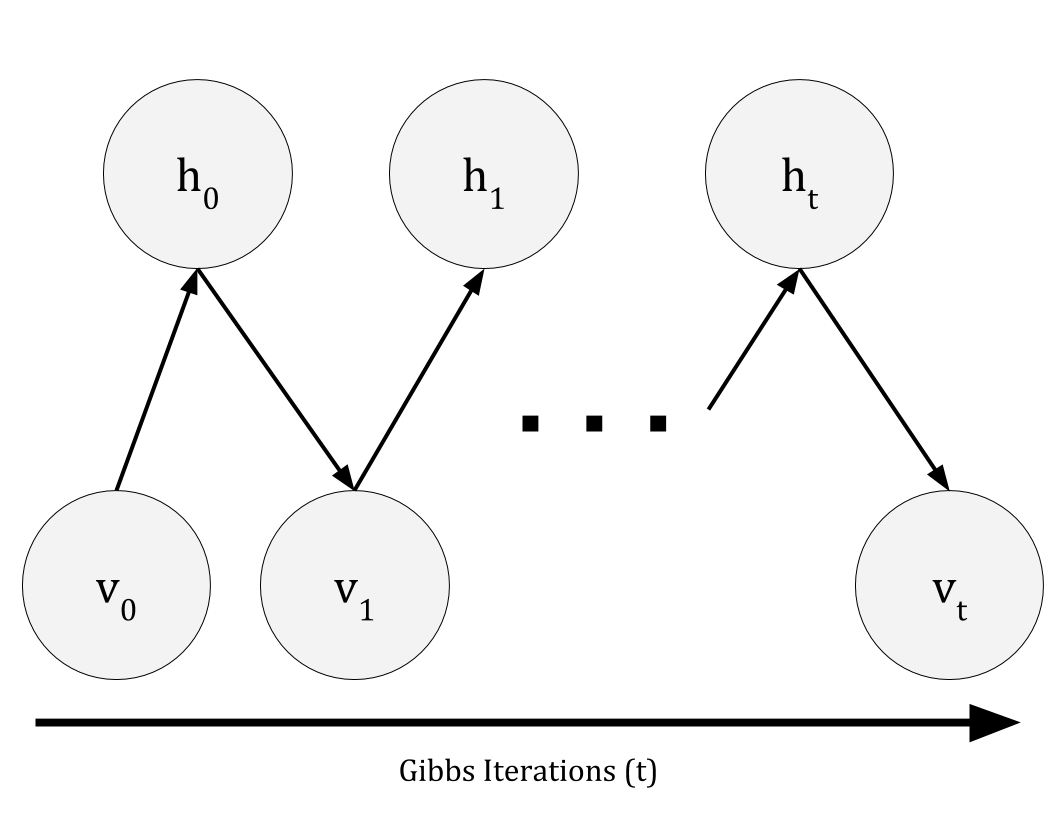
\includegraphics[width=0.48\textwidth]{Assets/Gibbs_Chain.png}
  \end{center}
  \caption{A figure illustrating a Gibbs chain where left to right indicates a Gibbs iteration. Note this is not a PGM.}
  \label{F:Gibbs_Chain}
\end{wrapfigure}

For the following discussion, the hidden units are indexed by $j$ and the visible units are indexed by $i$.

To perform Gibbs sampling in an RBM one must sample from $P(\tilde{h}|\tilde{v})$ giving a hidden state $\tilde{h}$. Using this hidden state a visible state is then generated, $\tilde{v'}$, by sampling from $P(\tilde{v'}|\tilde{h})$ and so on. This forms the Gibbs Chain \todocite{Feel like I could  cite this again in like a CD paper or something.} This process is visualised in figure \ref{F:Gibbs_Chain}

In a standard RBM, updating a hidden unit $h_j$ when performing Gibbs sampling is calculated by finding $ P(h_j = 1 | \tilde{v}) $ where $\tilde{v}$ is an input pattern. In the context of an image, $ \tilde{v} $ would be the pixel values where each pixel corresponds to a visible unit, $v_i$.
The probability of a given hidden unit activating in standard Gibbs sampling is: \todocite{Gibbs sampling would be good here}.
$$
P(h_j = 1 | \tilde{v}) = \sigma(\psi_j)
$$
Where $\psi_j$ is the weighted sum into the $jth$ hidden unit and $\sigma()$ is the Sigmoid function, or it also known as the Logistic function $\sigma(x)=1/(1+e^{-x})$. Figure \ref{F:PSI} \todowording{shows} psi for an example RBM.

\begin{figure}[h]
\begin{center}
  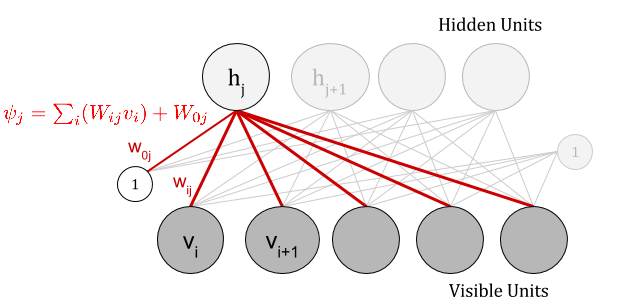
\includegraphics[width = 0.8\textwidth]{Assets/PSI_and_PHI.png}
\caption{A diagram showing $\psi_j$, the weighted sum into the $jth$ hidden unit.}
\label{F:PSI}
\end{center}
\end{figure}

As the weights are symmetric, sampling from the visible layer, given a hidden state is similar. That is $P(v_i = 1 | \tilde{h})$, where $\tilde{h}$ is the entire hidden vector is given by:
$$ P(v_i = 1 | \tilde{h}) = \sigma(\phi_{i}) $$
Where $\phi_i$ is the weighted sum into the $ith$ visible unit.

$$ \phi = \sum(W_{ji}h_{j}) + W_{0i} $$


\subsection{Unrolling a Gibbs Chain, a different perspective on RBM inference}

\begin{wrapfigure}{r}{0.6\textwidth}
  \begin{center}
    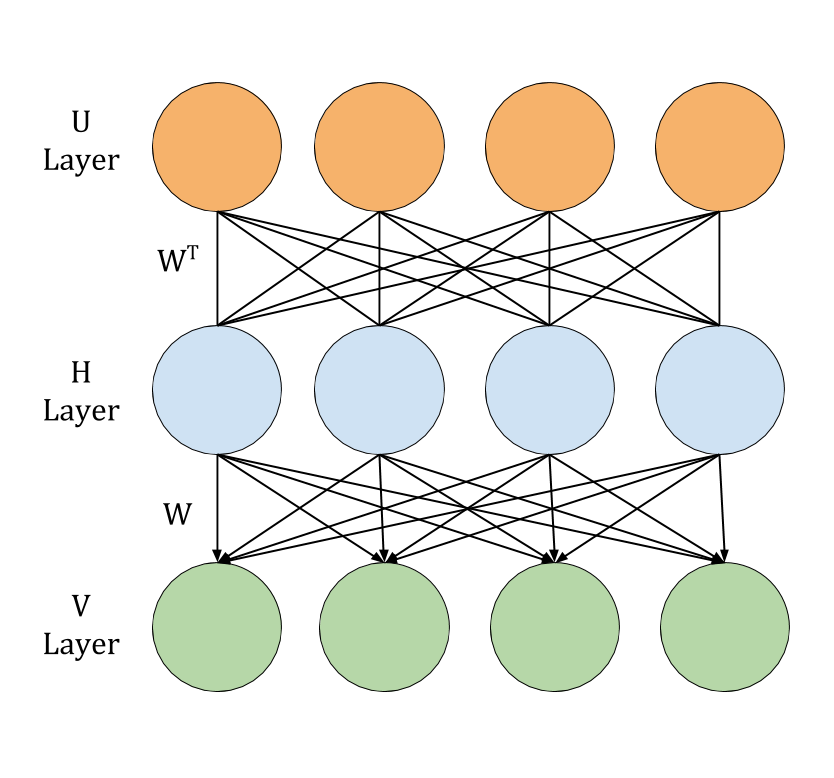
\includegraphics[width=0.5\textwidth]{Assets/3_Layer_RBM.png}
  \end{center}
  \caption{A diagram illustrating `unrolling` an RBM by one Gibbs iteration.}
  \label{F:3-Layer-RBM}
\end{wrapfigure}

Before the ORBMs architecture can be introduced, Gibbs sampling in an RBM must be presented in a different way. \todocite{Hintons paper on unrolling the Gibbs chain. He showed that RBM is infinitely deep belief network with tied weights}. This unrolling a single Gibbs iteration is illustrated in figure \ref{F:3-Layer-RBM}, the $U$ layer corresponding to the $V$ layer after one Gibbs iteration. To clarify, the $U$ layer corresponds to $v_1$ in figure \ref{F:Gibbs_Chain}.

Note the weights between the $H$ and $U$ layer are the transpose of the weights between the $V$ and $H$ layer.



We can show that Gibbs sampling in this RBM unrolled with a Sigmoid belief network is equivalent to Gibbs Sampling in a standard RBM.



\subsubsection{Ancestral Sampling in this equivalent network}

Ancestral sampling in an RBM \todocite{as described in the section where I talk about dreams...}. This network behaves a similar way, where a Gibbs chain is run between the top two layers, the $U$ and $H$ layer, until the last iteration. At the last iteration a hidden pattern is sampled and then is pushed through the Sigmoid belief network between $H$ and $V$. This is illustrated in figure \ref{F:3-Layer-RBM-Gibbs}.

\begin{figure}[h]
\begin{center}
  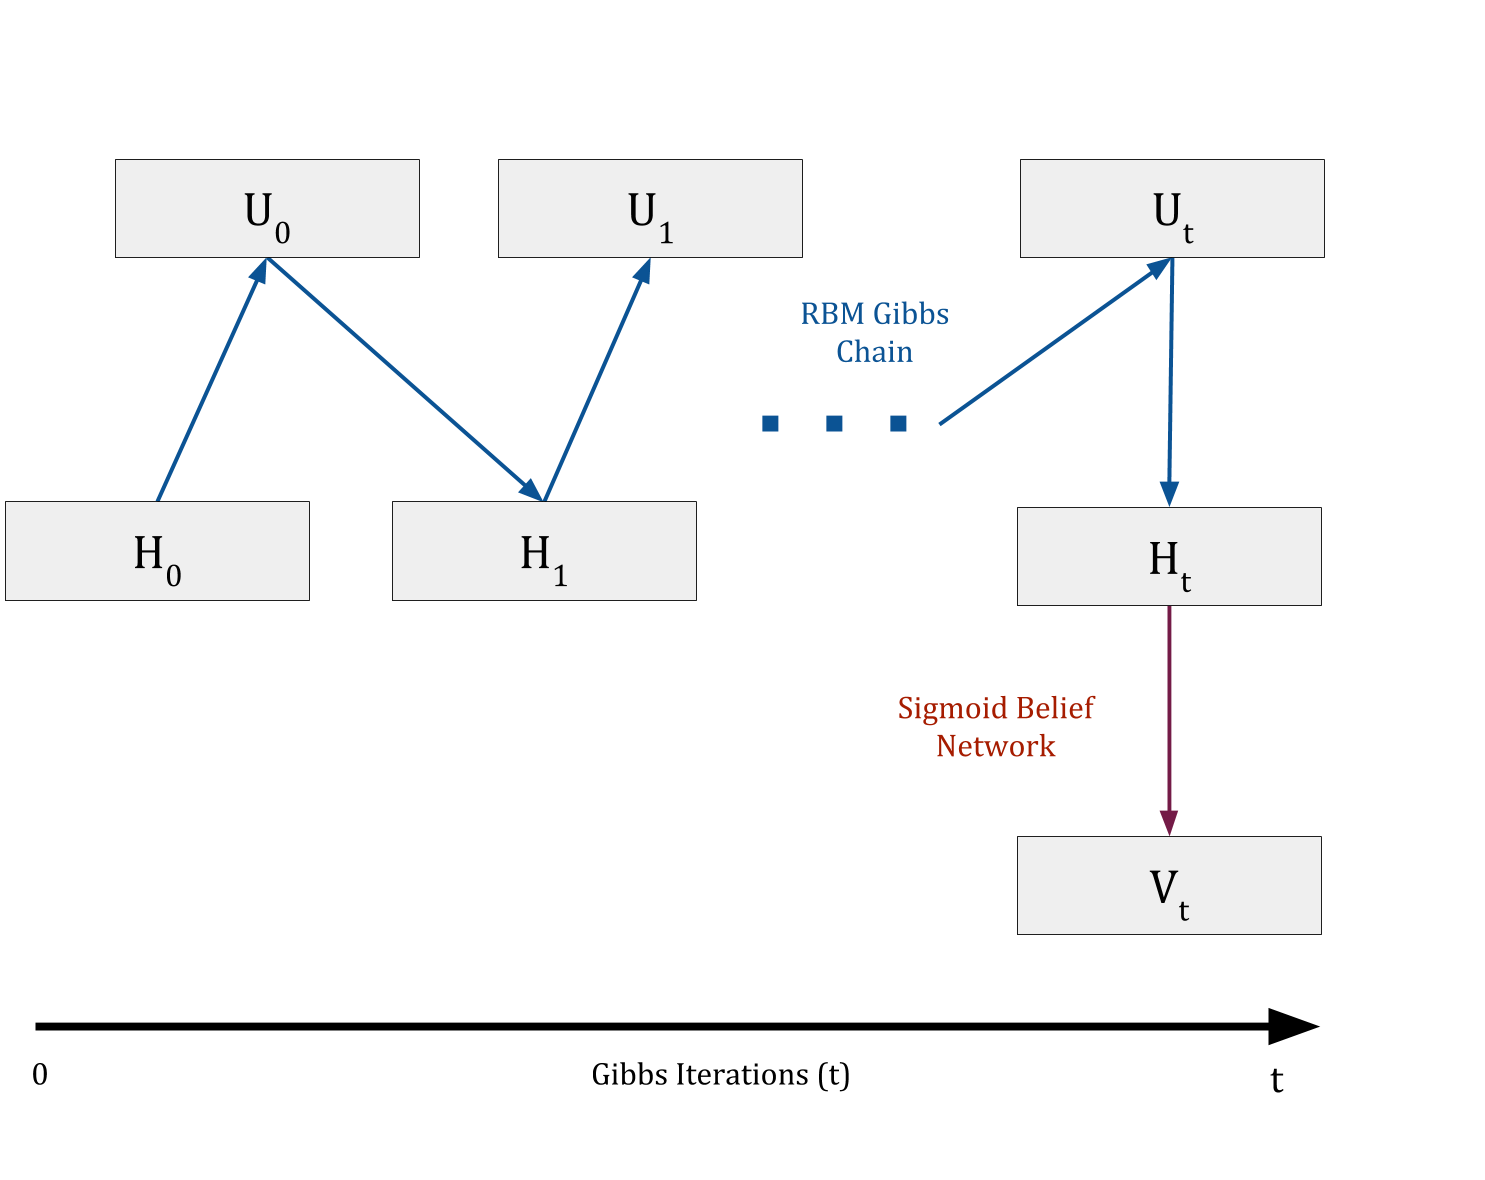
\includegraphics[width = 0.65\textwidth]{Assets/ORBM-Gibbs-Chain.png}
\caption{A diagram showing Ancestral sampling in the equivalent network, where normal sampling in the top 2 layers is performed until Gibbs iteration $t$ the hidden state is pushed through the bottom layers Sigmoid Network.}
\label{F:3-Layer-RBM-Gibbs}
\end{center}
\end{figure}

\todowording{We know (from above) how to generate the $h$ sample: Gibbs sampling from the RBM will do it. Then, the conditional probability of $v$ under a sigmoid belief net is (by definition) $p(v_i=1|h) = \sigma_i(h)$.
Thus Gibbs sampling from a simple RBM ending in a sample for $v$ is the same as sampling $h$ from the same RBM and then using a sigmoid belief net for the last step.}

\todowording{However, there's another way to draw such samples. Write (product rule) $\log P^\star(h,v) = \log P^\star(h) + \log P(v|h)$. We have the second term already:
$$ \log P(v|h) = \sum_i v_i \log \sigma_i(h) + (1-v_i) \log (1 - \sigma_i(h))$$}

To find $P^\star(h)$ we need to marginalise that joint over all $\mathbf{v}$ configurations:

$$
 \begin{aligned}
P^\star(h) &= \sum_{v_1=0}^1 \cdots \sum_{v_n=0}^1 \exp \bigg[  \log P^{\star}(h,v) \bigg] \\
&= \sum_{v_1=0}^1 \cdots \sum_{v_n=0}^1 \exp \bigg[  \sum_i  \sum_j h_j W_{ji} v_i \;\; + \;\; \sum_i W_{0i} v_i \;\; + \;\; \sum_j W_{j0} h_j \bigg] \\
&= \sum_{v_1=0}^1 \cdots \sum_{v_n=0}^1 \exp \bigg[  \sum_i v_i \phi_i(h)  \;\; + \;\; \sum_j W_{j0} h_j \bigg] \\
\text{where } \phi_i(h) &= \sum_j W_{ji} h_j + W_{0i} \\
&= \exp\left[ \sum_j h_j  W_{j0} \right] \;\; \times \sum_{v_1=0}^1 \cdots \sum_{v_n=0}^1 \prod_i \exp\bigg[ v_i \phi_i(h) \bigg] \\
&= \exp\left[\sum_j h_j  W_{j0}\right] \;\; \times \prod_i \bigg( 1 + e^{\phi_i(h) } \bigg) \\
\text{and so}
\log P^\star(h) &= \sum_j h_j  W_{j0} \;\; +  \sum_i \log \bigg( 1 + e^{\phi_i(h) } \bigg)
\\
&= \sum_j h_j  W_{j0} \;\; + \; \sum_i \phi_i(h) \;  - \; \sum_i \log \sigma_i(h)
\end{aligned}
$$

So far we've figured out $\log P^\star(h)$ for the RBM that is the `top layer`.

Therefore another way to write $\log P^\star(h,v)$ is
$$
\log P^\star(h,v) = \underbrace{\sum_j h_j  W_{j0} \;\; + \; \sum_i \phi_i(h) \;  - \; \sum_i \log \sigma_i(h)}_{\log P^\star(h)} \;\;+\;\; \underbrace{\sum_i v_i \log \sigma_i(h) + (1-v_i) \log (1 - \sigma_i(h))}_{\log P(v \mid h)}
$$
By collecting terms and simplifying one can readily those that this matches the earlier form \todocite{The earlier equation}.


\subsection{The ORBM architecture is derived from the equivalent RBM architecture}
This equivalent network can be extended to form the ORBMs architecture.

The design of the ORBM is such that two RBMs are used to model independant causes. As a generative model, the RBMs act independanlty, combining to form the visible pattern $\tilde{v}$. This is shown in figure \ref{F:ORBM-Architecture}. This architecture is simpler in practice as the U layers are factored out during the derivation.

\begin{figure}[h]
\begin{center}
  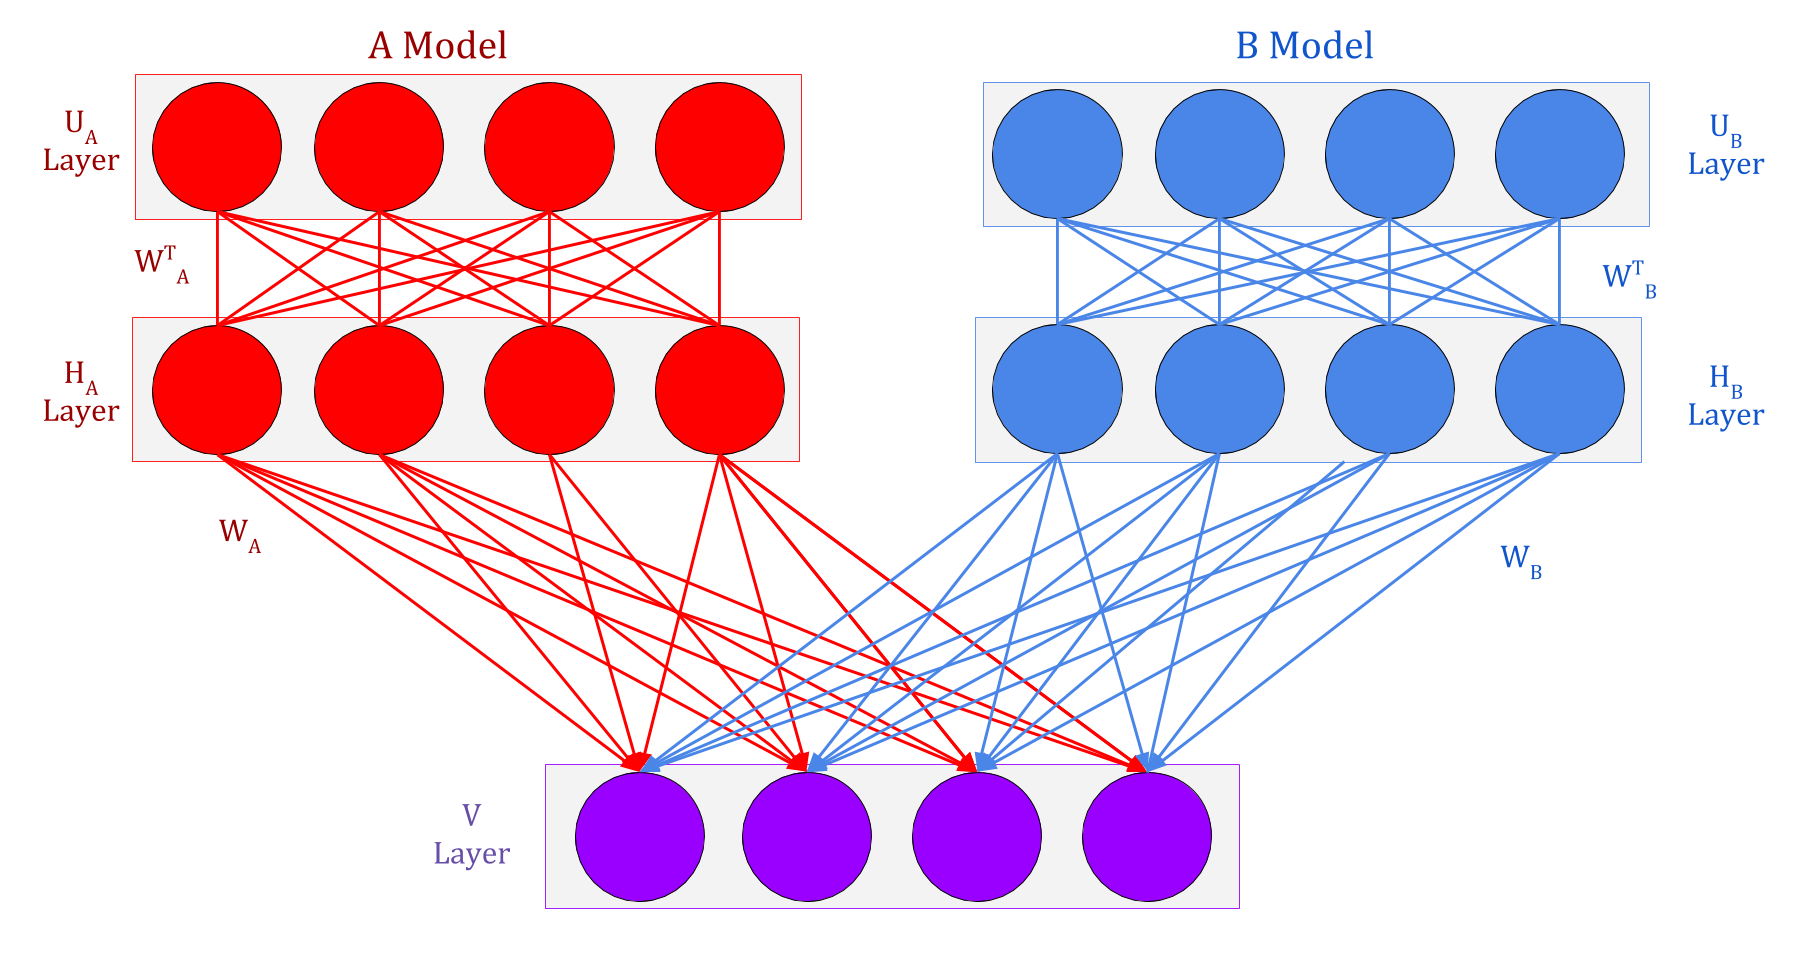
\includegraphics[width = 7in]{Assets/ORBM-Full-Architecture.png}
\caption{The full ORBM architecture, where $A$ and $B$ are the two causes that combine to form the data.}
\label{F:ORBM-Architecture}
\end{center}
\end{figure}

\subsection{Gibbs in a two cause model}

For reasoning about the two cause model of the ORBM it is useful to work in terms of RBM A and consider the input of the other RBM as $ \epsilon$.

\todowording{We're interested in how this will affect the Gibbs updates to the hidden units $h$ in the first RBM.}

\todowording{Note: $\epsilon_i $ is in general going to be a weighted sum of inputs from the second RBM's hidden layer, plus a new bias arising from the second RBM. Although the two biases both going into the visible units seems (and might be) redundant, in the generative model it seems sensible that visible activations under the two "causes" would have different background rates if taken separately (ie. different biases). So for now I think we should leave them in, but maybe hope to eliminate merge if possible in future, if it helps anything...}

\todowording{Before going on to the Gibbs Sampler version in which visible units are clampled, consider "ancestral" sampling from the model: each RBM independently does alternating Gibbs Sampling for a (longish) period, and then both combine to generate a sample $v$ vector, by adding both their weighted sums ($\phi$) and adding in both their visible biases too . That's a much more efficient way to do the "sleep" phase than doing what follows (which is mandatory for the "wake" phase samples however).}

The Gibbs update step is given by $p_j = \sigma(\phi_j) $ with
$ \psi_j = \log P^*(h,v ; h_j =1 ) - \log P^*(h,v ; h_j = 0)$.

However this time we don't have exact correspondence with an RBM because only the final step involves $\epsilon$, not the reverberations in the RBM above it that generates $h$. So it's not enough to consider just the RBM alone, with it's joint being just the product of factors in the first line of math above. We need to incorporate the last step explicitly, with its slight difference in the form of $\phi^B_i$. We know the joint decomposes into this:
$$ \log P^* (h,v) = \log P^*(h) + \log P(v|h)$$
where the first term is the vanilla RBM probability but the second is the final layer's probability, now given by
$$ \log P(v|h^A,h^B) = \sum_i v_i \log \sigma (\phi^A_i(h) + \phi^B_i) + (1-v_i) \log (1 - \sigma(\phi^A_i(h) + \phi^B_i)$$

To carry out Gibbs sampling in the hidden layer of this architecture we need to calculate $\psi^A_j = \log P^*(h,v ; h^A_j =1 ) - \log P^*(h,v ; h^A_j = 0)$. We'll use the fact that $\phi^A_i(h ; h^A_j=1) = \phi^A_i(h ; h^A_j=0) + W^A_{ji}$.

And we'll abbreviate $\phi^A_i(h ; h_j=0)$ to $\phi^{Aj0}_i$.

We obtain:
$$\psi^A_j = \sum_i v_i \log \left( \frac{1+ e^{-\phi^{Aj0}_i - \phi^B_i}}{1+e^{-\phi^{Aj0}_i - W_{ji} -\phi^B_i}} \frac{1+ e^{\phi^{Aj0}_i + W_{ji} + \phi^B_i}}{1+e^{\phi_i^{Aj0} + \phi^B_i}}\right) \;\;+ \;\;\sum_i \log \left(\frac{1+e^{\phi_i^{Aj0} + W_{ji}}}{1+ e^{\phi_i^{Aj0}}}
\frac{1+e^{\phi_i^{Aj0} + \phi^B_i}}{1+ e^{\phi_i^{Aj0} + W_{ji} + \phi^B_i}} \right)
$$

Now $\phi = \log \frac{1+e^{\phi}}{1+e^{-\phi}}$ (Marcus' magic identity), which is$ = \log \frac{\sigma(\phi)}{\sigma(-\phi)}$.
So the first term simplifies to
$ \sum_i v_i W_{ji}$, which is the same as that in a "vanilla RBM".

The second term can also be simplified, using the identity $\log(1-\sigma(\phi)) = \phi - \log(1+e^\phi)$.

This leads to the following Gibbs Sampler probability of the j-th hidden unit in network $A$ being 1: $p_j = \sigma(\psi_j^A)$ with

$$\psi_j^A = \underbrace{\sum_i W^A_{ji} v_i}_\text{vanilla RBM} \; + \; \underbrace{\sum_i C^A_{ji}}_\text{correction} $$
where
$$
\begin{aligned}
C^A_{ji} \; &= \;\log \bigg[ \frac{\sigma (\phi_i^{Aj0})}{\sigma (\phi_i^{Aj0} + W^A_{ji})} . \frac{\sigma (\phi_i^{Aj0} + W_{ji}^A + \phi_i^B) }{\sigma (\phi_i^{Aj0} + \phi_i^B)} \bigg]
\\
&= \log \sigma(\phi_i^{Aj0})  \; + \; \log \sigma (\phi_i^{Aj0} + W^A_{ji} + \phi_i^B) \;- \log \sigma (\phi_i^{Aj0} + W^A_{ji})  \; - \; \log \sigma ( \phi_i^{Aj0} + \phi_i^B)
\\
&= \log \bigg[ \frac{\sigma(\phi_i^{A} - h^A_i W^A_{ji})}{\sigma (\phi_i^{A} + (1-h^A_i) W^A_{ji})} \bigg]  \; - \; \log \bigg[ \frac{ \sigma ( \phi_i^{AB} - h^A_i W^A_{ji})}{\sigma (\phi_i^{AB} + (1-h^A_i) W^A_{ji})} \bigg]
\end{aligned} $$

where $\phi_i^{AB} = \phi_i^{A} + \phi_i^{B}$.

Notice that, weirdly enough, $v$ plays no role in this correction!

It is clear that adding $\phi^B_i$ has introduced a dependency between the whole of $h$, which is "a bit of a worry".

\todowording{The majority of this...}

\subsection{Approximating the Correction}

\begin{figure}[h]
\begin{center}
  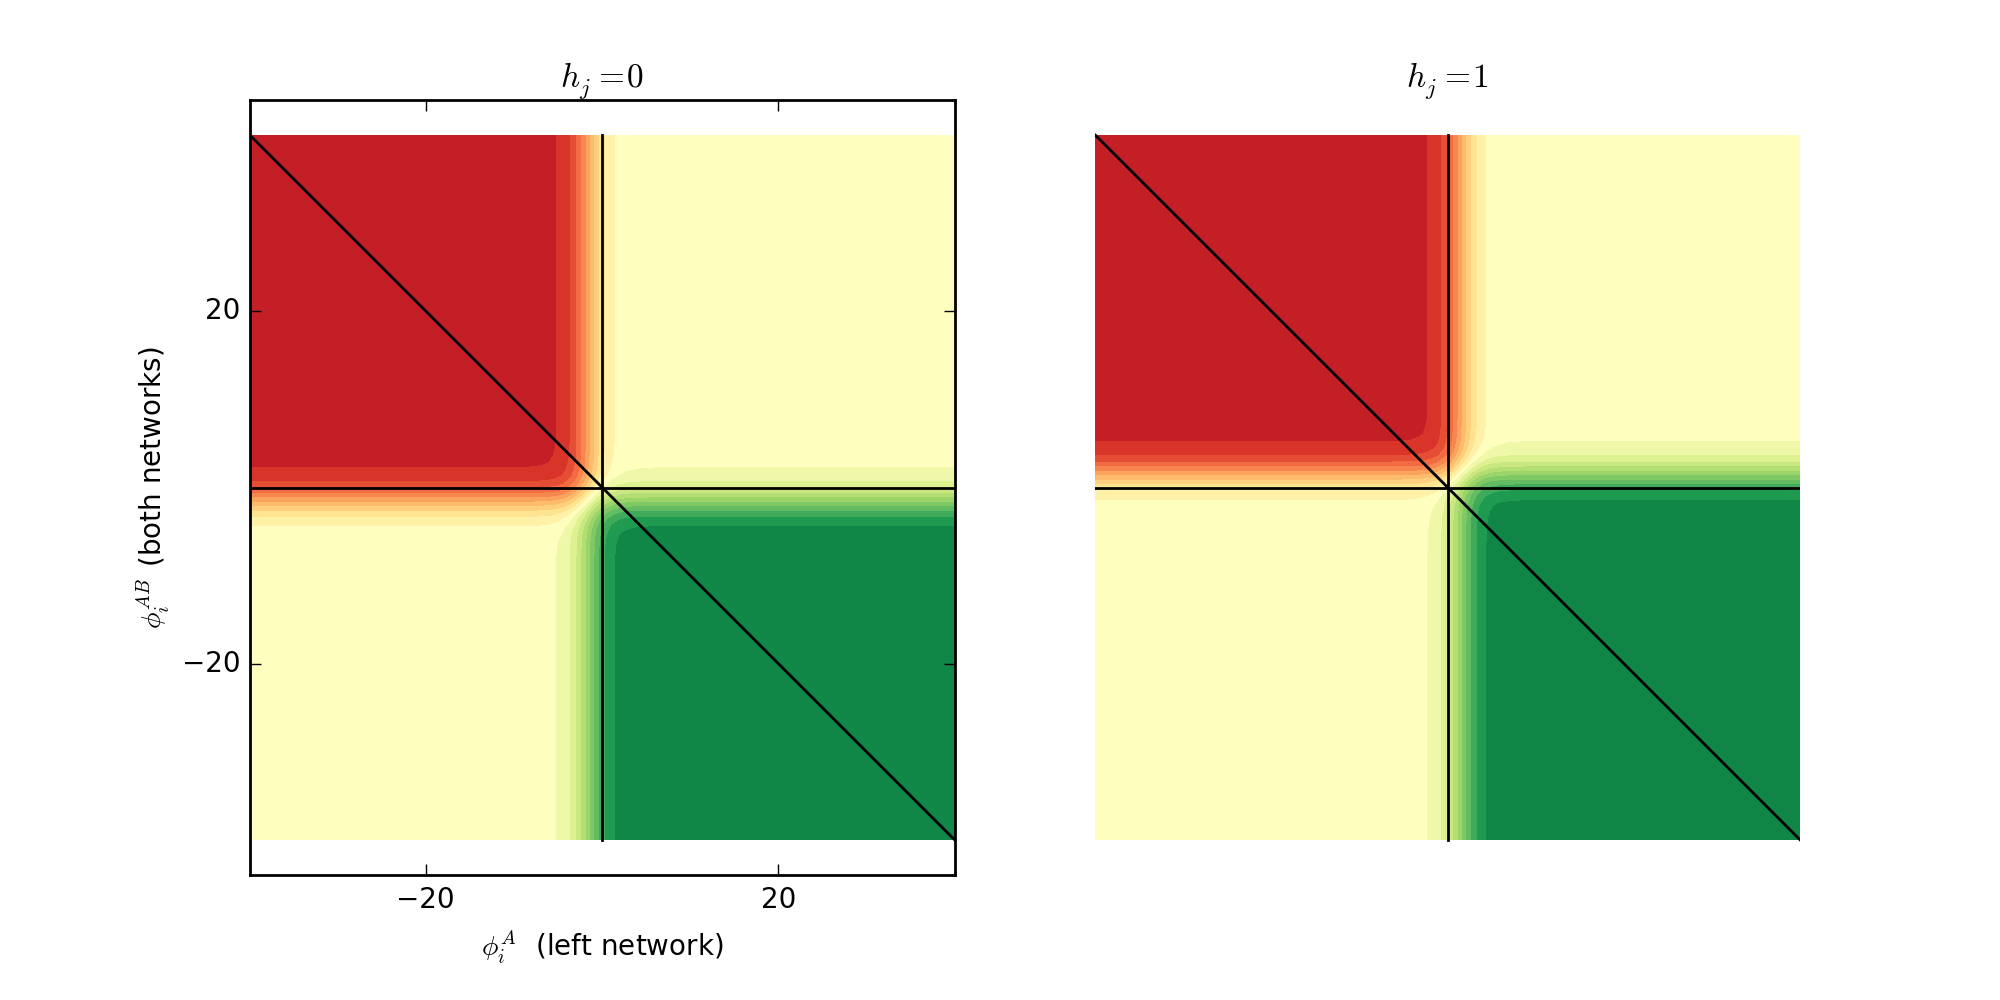
\includegraphics[width = 0.65\textwidth]{Assets/correction.png}
\caption{A diagram what the correction function looks like for ...}
\label{F:Correction-Plot}
\end{center}
\end{figure}

% \subsection{}
%
%
% The difference in architecture from an RBM means that a slightly different inference algorithm is required, as the representations are represented separately for a composite input.
%
% \begin{itemize}
%   \item Inference in this generative model is P(ha, hb given v) , we want to represent the causes separately.
%
%   \item Unfornately, ha and hb are dependant given the visible v. meaning to perform inference, obtaining a hidden representation requires a Gibbs chain
%   \item Diagram showing the inference gibbs chain.
%
% \end{itemize}
%
%
% \subsubsection{Calculating the Posterior}
%
% To find the $ P(h_a, h_b | v_{comp}) $, where $h_a$ and $h_b$ are the separate representations of the data caused $a$ and $b$, and $v_{comp}$ is the composed/composite input. We must sample from a Gibbs Chain,  as $h_a$ and $h_b$ are dependant given $v_{comp}$. This ends up being almost identical to the RBM except we add a 'Correction', when computing the update for $h_a$ and $h_b$ respectively.
%
% TODO-SHOW-THE-FULL-CORRECTION
%
% \subsection{Source Separation - Reconstructions in the ORBM}
%
% To actually perform source separation, one needs to simply take the internal representation generated by the inference step, and generate a visible pattern in the same way you would with a standalone RBM.
